% % % % % % % % % % % % % % 
% 
% Skript zu NUMERIK I
% WS14/15
% von Prof. Dr. Blank
% Universität Regensburg
% 
% 
%	Kap. 7: Numerische Integration/Quadratur
% 
% % % % % % % % % % % % % % 

\chapter{Numerische Integration/Quadratur}

\sectione{Einführung und einfache Quadraturformeln}
Häufig sind Integrale
\begin{gather*}
  I(f) \coloneqq \int_a^bf(t)\dd t
\end{gather*}
nicht analytisch zu berechnen
oder die benötigte analytische Darstellung
des unbestimmten Integrals ist kompliziert.
Ziel ist $I(f)$ durch eine 
\textbf{Numerische Quadratur}\index{Numerische Quadratur}
$\hat{I}(f)$ zu approximieren.

Der Begriff numerische Integration ist allgemeiner und
beschreibt das numerische Lösen von
\begin{gather*}
  y'(t) = f\big(t,y(t)\big) \qquad \text{mit } y(a)=c
\end{gather*}
Die numersiche Quadratur $\hat{I}(f)$ sollte
\begin{enumerate}[a)]
\item effizient ausführbar sein,
\item viele Eigenschaften der Integration beibehalten und
\item $I(f)$ gut approximieren.
\end{enumerate}
Zur Wiederholung einige Eigenschaften des Riemann-Integrals:\\
Seien $f,g\in C([a,b])$, dann ist $I\colon C([a,b])\to\R$
eine positive Linearform, d.h. $I$ ist linear und 
\begin{gather}
  f\geq 0 \quad \Rightarrow \quad I(f)\geq 0
  \label{VII.1.1}
\end{gather}
Weiterhin gilt
\begin{gather}
  \int_a^b f(t)\dd t + \int_b^c f(t)\dd t = \int_a^cf(t)\dd t
  \label{VII.1.2}
\end{gather}
Diese sollen nun möglichst beibehalten werden.

\begin{Defe}\label{7.1.1}
  Ein Verfahren heißt konvergent von der Ordnung $p$
  (hat die Konvergenzordnung $p$),
  falls der Fehler (hier $|I(f)-\hat{I}(f)|$)
  mit $\mathcal{O}(h^p)$ gegen Null geht für $h\to 0$.
\end{Defe}

\subsectione{Mittelpunktregel}
\imagemissing{Veranschaulichung der Mittelpunktregel}\label{im7.1.2}
Zerlege $[a,b]$ in Teilintervalle $[x_i,x_{i+1}]$
für $i=0,\dotsc,n-1$ der Länge $h_i=x_{i+1}-x_i$, d.h.
$a=x_0 < x_1 < \dotsb < x_n = b$,
und setze zur Approximation von $I(f)$
\begin{gather}
  \hat{I}_M(f) \coloneqq \sum_{i=0}^{n-1}f\left(
    \frac{x_{i+1}+x_i}{2}
  \right)
  \cdot (x_{i+1}-x_i)
  \label{VII.1.3}
\end{gather}
Für ein äquidistantes Gitter ergibt sich mit $h=\frac{b-a}{n}$
\begin{gather}
  \hat{I}_M(f)= h \sum_{i=0}^{n-1}f\left(
    x_{i}+\frac{h}{2}
  \right)
  \label{VII.1.4}
\end{gather}
Die \textbf{Fehlerschranke}\index{Fehlerschranke}
(Konvergenzordnung) für $f\in C^2([a,b])$
\begin{gather}
  \left| I(f) -\hat{I}_M(f)\right|
  \leq \frac{h^2}{24}(b-a)\nn[f'']_\infty
  \label{VII.1.5}
\end{gather}
ergibt sich aus der Taylorentwicklung
\begin{gather*}
  f(t) = f\left(x_i+\frac{h}{2}\right)
  + f'\left(x_i+\frac{h}{2}\right) \cdot 
  \left(t-\left(x_i+\frac{h}{2}\right)\right)
  + \frac{1}{2}f''\big(\xi_i(t)\big)\cdot
  \left(t-\left(x_i+\frac{h}{2}\right)\right)^2
\end{gather*}
mit einer Zwischenstelle $\xi_i(t)$ zwischen $t$ und
$\left(x_i+\frac{h}{2}\right)$, denn
\begin{align*}
  \left|I(f)-\hat{I}_M(f)\right|
  &\leq \sum_{i=0}^{n-1} \left|
    \int_{x_i}^{x_{i+1}}f(t)\dd t - h\cdot f\left(x_i+\frac{h}{2}\right)
    \right|\\
  &=\sum_{i=0}^{n-1} \left|
    \int_{x_i}^{x_{i+1}}\left( 
    f(t) - f\left(x_i+\frac{h}{2}\right)
    \right) \dd t
    \right|\\
  &= \sum_{i=0}^{n-1} \left|
    \int_{x_i}^{x_{i+1}}
    f'\left(x_i+\frac{h}{2}\right) \cdot 
    \left(t-\left(x_i+\frac{h}{2}\right)\right)
    + \int_{x_i}^{x_{i+1}}
    f''\big(\xi_i(t)\big)
    \cdot \left(t-\left(x_i+\frac{h}{2}\right)\right)^2\dd t
      \right|\\
  \intertext{
    da $\int_{x_i}^{x_{i+1}}\left(
    t-\left(x_i+\frac{h}{2}\right)
    \right)\dd t=0$
    }
  &= \sum_{i=0}^{n-1} \left|
    \int_{x_i}^{x_{i+1}}
    \frac{1}{2} f''\big(\xi_i(t)\big)
    \cdot \left(t-\left(x_i+\frac{h}{2}\right)\right)^2\dd t
    \right|\\
  &\leq \nn[f'']_\infty \cdot \frac{1}{2}
    \sum_{i=0}^{n-1}
    \int_{x_i}^{x_{i+1}}
    \left(t-\left(x_i+\frac{h}{2}\right)\right)^2\dd t\\
  &= \nn[f'']_\infty \cdot \frac{1}{2}
    \sum_{i=0}^{n-1}
    \frac{1}{3}\left[
    x_{i+1}\left(\underbrace{x_{i+1}-x_i}_{h}-\frac{h}{2}\right)^2
    - x_{i}\left(x_{i}  -x_i-\frac{h}{2}\right)^2
    \right]\\
  &= \nn[f'']_\infty \frac{h^2}{24}
    \cdot \sum_{i=0}^{n-1} (x_{i+1}-x_i)\\
  &=\frac{h^2}{24} (b-a)\nn[f'']_\infty
\end{align*}
Für andere Interpolationspunkte als den Mittelpunkt 
(z.B. einer der Eckpunkt) wird $\mathcal{O}(h^2)$, d.h. 
die Ordnung $2$, nicht erreicht.

\subsectione{Trapezsumme}
Für die Trapezsumme wird stückweise stückweise linear interpoliert.
\imagemissing{Veranschaulichung Trapezsumme}\label{im7.1.3}
Mit der \textbf{Trapezregel}\index{Trapezregel}
$(x_{i+1}-x_i)\cdot \frac{f(x_i)+f(x_{i+1})}{2}$
ergibt sich
\begin{gather}
   \hat{I}_T(f) = \frac{1}{2}\sum_{i=0}^{n-1}
    \big(
    f(x_i)+f(x_{i+1})
    \big)
    \cdot (x_{i+1}-x_i)
    \label{VII.1.6}
\end{gather}
und für äquidistante Gitter wird dies zur 
\textbf{Trapezsumme}\index{Trapezsumme}
\begin{gather}
  \hat{I}_T(f) = h\cdot\left( \frac{1}{2}f(x_0)
    +\sum_{i=0}^{n-1}f(x_i)
    +\frac{1}{2} f(x_n)
  \right)
  \label{VII.1.7}
\end{gather}
Die Konvergenz folgt durch die Riemannschen Unter- bzw. Obersummen
$R_u^{(k)}(f)$ und $R_o^{(k)}(f)$ wegen
\begin{gather*}
  I(f)\longleftarrow R_u^{(k)}(f)
  \leq \hat{I}_T(f)
  \leq R_o^{(k)}(f)\longrightarrow I(f)
  \qquad \text{für } h\to 0
\end{gather*}
Später zeigen wir noch die Konvergenzordnung für $f\in C^2([a,b])$
\begin{gather}
  \left| I(f)-\hat{I}_T(f)\right| \leq \frac{h^2}{12}(b-a)\nn[f'']_\infty
  \label{VII.1.8}
\end{gather}
Offensichtlich erfüllen $\hat{I}_M(f)$ und $\hat{I}_T(f)$
die Eigenschaften aus \ref{7.1.1}.
Weiterhin sind sie für lineare Funktionen exakt,
d.h. berechnen die genauen Integralwerte.


\sectione{Interpolatorische Integrationsformeln}
\index{Integrationsformel!interpolatorische/Newton-Cotes-Formeln}
(auch Newton-Cotes-Formeln)\\
Die Idee ist nun, $f$ auf $[a,b]$ polynomial zu interpolieren
an verschiedenen Stellen $a\leq x_0\leq x_1\leq \dotsb\leq x_n<b$
und dann das Integral zu berechnen, d.h.
\begin{align}\nonumber
  \hat{I}(f) &\coloneqq I\big( \ipol{p}{f}{x_0,\dotsc,x_n}\big)\\\nonumber
             &=\sum_{i=0}^{n}f(x_i)
               \cdot \int_a^bL_i(t)\dd t\\
             &=\sum_{i=0}^{n} w_if(x_i)
               \label{VII.2.1}
\end{align}
mit den Gewichten\index{Gewichte!Newton-Cotes-}
\begin{gather}
  w_i\coloneqq \int_a^bL_i(t)\dd t\, .
  \label{VII.2.2}
\end{gather}
Offensichtlich sind diese Quadraturformeln exakt
für Polynome vom Grad weniger oder gleich $n$.

Es gilt sogar
\begin{Leme}\label{7.2.1}
  Zu $n+1$ paarweise verschiedenen Knoten $x_0,\dotsc, x_n$
  gibt es genau eine Quadraturformel
  \begin{gather*}
    \hat{I}(f) = \sum_{i=0}^nw_if(x_i)
  \end{gather*}
  mit $w_i\in\R$, welche für alle Polynome $p\in\p_n$ exakt ist.

  \begin{proof}
    $L_i\in\p_n$, also 
    \begin{gather*}
      I(L_i)=\hat{I}(L_i)=\sum_{j=0}^{n}w_jL_i(x_j)
                         =\sum_{j=0}^{n}w_j\delta_{ij}
                         =w_i \quad \text{für } i=0,\dotsc,n
    \end{gather*}
    Die Gewichte sind damit eindeutig bestimmt.
  \end{proof}
\end{Leme}

\begin{Defe}\label{7.2.2}
  $\hat{I}$ heißt \textbf{abgeschlossene Quadraturformel}
  \index{Quadraturformel!abgeschlossen},
  falls $a=x_0$ und $b=x_n$.
  $\hat{I}$ heißt \textbf{offen}, falls $a<x_0$ und $x_n<b$.\\
  ($\hat{I}_M$ ist also eine offene Quadraturformel.)
\end{Defe}

\subsectione{Newton-Cotes-Formeln}
Abgeschlossene, interpolatorische Quadraturformeln mit
äquidistanter Stützstellenverteilung $x_0, \dotsc, x_n$ heißen
\textbf{Newton-Cotes-Formeln der Ordnung $n$}.
Mit $h=\frac{b-a}{n}$, $x_i=a+i\cdot h$ und Substitution
$z\coloneqq \frac{t-a}{h}$ gilt
\begin{gather}
  w_i\coloneqq h
  \cdot \int_0^n \prod_{\substack{j=0\\j\neq i}}^n\frac{z-j}{i-j}dz\, .
  \label{VII.2.3}
\end{gather}
Diese sind unabhängig von der Lage der Stützstellen
und liegen in Form von
\begin{gather*}
  w_i=\frac{b-a}{n\cdot s}\sigma_i
\end{gather*}
tabellarisch vor.  Es gilt $n\cdot s$, $\sigma_i\in\Z$ und
\begin{gather}
  \hat{I}_n(f) = \frac{(b-a)}{n\cdot s}
  \cdot \sum_{i=0}^{n}\sigma_i f(x_i)\,.
  \label{VII.2.4}
\end{gather}
Da sie exakt sind für $p\in \p_n$,
können $\frac{\sigma_i}{n\cdot s}$ z.B. aus dem
linearen Gleichungssystem für $[a,b]=[0,1]$
\begin{gather*}
  \int_0^1x^k\dd x=\frac{1}{n\cdot s}\sum_{i=0}^{n}\sigma_ix_i^k
  \qquad \text{für } k=0,\dotsc,n
\end{gather*}

\subsectione{Tabelle (Newton-Cotes-Gewichte)}
\index{Gewichte!Newton-Cotes-}
\begin{align*}
  \begin{array}{cccccccl}
    n\backslash \sigma_i &\sigma_1&\dots&&&& n\cdot s\\
    1 & 1&1&&&&2& \text{Trapezregel}\\
    2&1&4&1&&&6 & \text{Simpson-Regel}\\
    3&1&3&3&1&&8& \text{$\frac{3}{8}$-Regel}\\
    4&7&32&12&32&7&90 & \text{Milne-Regel}\\
    \vdots\\
    8&&&\dots &-4540&\dots
  \end{array}
\end{align*}
Positive Funktionen haben kein positives Integral ab einem $n_0$!!


% -------------------------------------------------


\marginpar{07.01.2015}
Daraus folgt, dass die Monotonie (Positivität) 
bei abgeschlossenen Newton-Cotes Formeln i.A. nicht gewährleistet ist,
wenn Polynome von hohem Grad exakt integriert werden sollen.
Diese sind dann daher ungeeignet.


\begin{Satze}\label{7.2.5}
  Sei $\hat{I}_n(f) $ die abgeschlossene Newton-Cotes-Formel
  der Ordnung $n$.
  Dann gilt
  \begin{enumerate}[a)]
  \item $\sum_{i=0}^nw_i= b-a$
  \item $w_i=w_{n-i}$
  \item Ist $n$ gerade, so ist $\hat{I}_n$ exakt für Polynome bis zum
    Grad $n+1$ nicht nur $n$.
  \end{enumerate}

  \begin{proof} siehe Übungsblatt \end{proof}
\end{Satze}

\begin{Satze}
  Sei $\hat{I}(f)\coloneqq \sum_{i=0}^n w_if(x_i)$ mit $w_i\in\R$ und
  $a\leq x_0<x_1<\dotsb <x_n\leq b$.
  Dann ist der Integrationsfehler $R$ mit 
  \begin{gather}
    R(f) \coloneqq \hat{I}(f) - \int_a^b f(x) \dd x
    \label{VII.2.5}
  \end{gather}
  eine lineare Abildung, für die folgende Darstellungsformel gilt:
  Falls $R(p)=0$ für alle $p\in\p_l$, dann gilt 
  für alle $f\in C^{l+1}([a,b])$
  \begin{gather}
    R(f) = \int_a^bf^{(l+1)}(t) K(t) \dd t
    \label{VII.2.6}
  \end{gather}
  mit 
  \begin{align}\nonumber
    K(t) &\coloneqq \frac{1}{l!}
           R\left( 
           (\bullet -t)_+^l
           \right)\\
         &= \frac{1}{l!}\left( 
           \sum_{i=0}^n w_i(x_i-t)_+^l-\int_a^b(x-t)_+^l\dd x  
           \right)
           \label{VII.2.7}
  \end{align}
  $K(t)$ heißt \textbf{Peano-Kern des Funktionals
    $R$}\index{Peano-Kern}.
  \begin{proof}
    Es gilt
    \begin{gather*}
      f(x) = f(a) + f'(a)(x-a) +\dotsb + \frac{f^{(l)}(a)}{l!}(x-a)^l + r_l(x)
    \end{gather*}
    mit Restglied 
    \begin{align*}
      r_l(x) &= \frac{1}{l!} \int_a^xf^{(l+1)} (t)\cdot (x-t)^l \dd t\\
             &= \frac{1}{l!} \int_a^bf^{(l+1)} (t)\cdot (x-t)_+^l \dd t
    \end{align*}
    Da $R(p)=0$ für alle $p\in\p_l$ folgt
    \begin{align*}
      R(f) &= R(r_l)
             = \frac{1}{l!} R\left(\int_a^bf^{(l+1)} (t)\cdot(\bullet-t)_+^l
             \dd t\right)\\
           &=\frac{1}{l!}\left\{ \sum_{i=0}^n w_i \int_a^b f^{(l+1)}(t)
             \cdot (x_i-t)_+^l\dd t  
             - \int_a^b\int_a^b  f^{(l+1)}(t) \cdot (x-t)_+^l\dd t\dd x  \right\}
    \end{align*}
    Mit dem Satz von Fubini gilt
    \begin{align*}
      R(f) &= \frac{1}{l!}\int_a^bf^{(l+1)}(t) 
             \left\{ 
             \sum_{i=0}^n w_i  \cdot (x_i-t)_+^l  
             - \int_a^b(x-t)_+^l\dd x  \right\}
             \dd t\\
           &= \frac{1}{l!} \int_a^bf^{(l+1)}(t) 
             \cdot R\left( (\bullet -t)_+^l\right) \dd t    
    \end{align*}
  \end{proof}
\end{Satze}

\begin{Fole}\label{7.2.7}
  Falls der Peano-Kern $K$ auf $[a,b]$ ein konstantes Vorzeichen hat,
  gilt nach dem Mittelwertsatz der Integralrechnung
  \begin{gather}
    R(f) = f^{(l+1)}(\xi) \int_a^b K(t)\dd t 
    \quad \text{für ein }\xi\in (a,b)
    \label{VII.2.8}
  \end{gather}
  Wähle nun ein $g$, für das $R(g)$ und $g^{(l+1)}$ bekannt oder leicht
  berechenbar sind, z.B.
  $g(x)\coloneqq x^{l+1}$. Hier ist
  \begin{gather*}
    \int_a^bK(t)\dd t = \frac{R(g)}{(l+1)!} = \frac{R(x^{l+1})}{(l+1)!}
  \end{gather*}
  Dann gilt für ein beliebiges $f\in C^{l+1}([a,b])$
  \begin{gather}
    R(f) = \frac{R(x^{l+1})}{(l+1)!} f^{(l+1)}(\xi)
    \quad \text{für ein }\xi \in (a,b)
    \label{VII.2.9}
  \end{gather}
\end{Fole}

\begin{Satze}[Approximationsfehler]\index{Newton-Cotes-Formeln!Fehler}
  Im Fall der Newton-Cotes-Formeln besitzen die Peano-Kerne
  konstante Vorzeichen. Somit gilt für $f\in C^{n+j+1}$ mit 
  $j= \begin{cases}
    0 & \text{für $n$ ungerade}\\
    1 & \text{für $n$ gerade}
  \end{cases}$
  \begin{gather}
    R_n(f) = \hat{I}_n (f) - \int_a^b f(x) \dd x
           = \frac{R(x^{n+j+1})}{(n+j+1)!}f^{(n+j+1)}(\xi)
             \label{VII.2.10}
  \end{gather}

  \begin{proof}
    Der Beweis des konstanten Vorzeichens gilt
    \cite[siehe][]{steffensen}.
    Nach Satz \ref{7.2.5}c) gilt
      $R_n(p) = 0 ~\forall p\in\p_{n+j}$.
    Mit \eqref{VII.2.9} und $l=n+j$ folgt dann die Aussage \eqref{VII.2.10}
  \end{proof}
\end{Satze}


\subsectione{Tabelle: Fehler für Newton-Cotes-Formeln}
\begin{gather*}\label{7.2.9}
  \begin{array}{cll}
    n & & R_n(f)\\
    1 &\text{Trapezregel} &(b-a)^3\cdot\frac{1}{12}f^{(2)}(\xi)\\
    2 &\text{Simpsonregel}&\frac{(b-a)}{2}^5\cdot\frac{1}{90}f^{(4)}(\xi)\\
    3 &\text{$\frac{3}{8}$-Regel}&\frac{(b-a)}{3}^5\cdot\frac{3}{80}f^{(4)}(\xi)\\
    4 &\text{Milne-Regel}
        &\frac{(b-a)}{4}^7\cdot\frac{8}{945}f^{(6)}(\xi)\\
  \end{array}
\end{gather*}

Die Erhöhung des Polynomgrades $n$
ergibt also
i.A. keine bessere Approximation.
Dies hängt auch von der Länge des
Intervalls $[a,b]$ ab.
Stattdessen werden die
Newton-Cotes-Formeln auf
Teilintervalle angewendet, 
d.h. sie bilden die Grundlage für
stückweise polynomiale
interpolatorische Integrationsformeln.

\subsectione{Iterierte (wiederholte)
  Newton-Cotes-Formeln}
\index{Newton-Cotes-Formeln!wiederholt}
Betrachte die Intervallunterteilung 
$a=t_0<t_1<\dotsb<t_N=b$ und approximiere
\begin{gather*}
  I(f) = \sum_{l=0}^{N-1}\int_{t_l}^{t_{l+1}}f(t)\dd t
\end{gather*}
durch wiederholtes Anwenden einer Newton-Cotes-Formel
$\hat{I}_n(f)$ auf die Teilintervalle $[t_l, t_{l+1}]$
(die Formel hier sei $\hat{I}_n^{(l)}(f)$),
d.h.
\begin{gather}
  \hat{I}(f) = \sum_{l=0}^{N-1}\hat{I}_n^{(l)}(f)
  = \sum_{l=0}^{N-1}\frac{t_{l+1}-t_l}{n\cdot s}
  \sum_{i=0}^n \sigma_i f(t_l+i\widetilde{h}_l)
  \label{VII.2.11}
\end{gather}
mit $\widetilde{h}_l\coloneqq (t_{l+1}-t_l)\cdot \frac{1}{n}$.
Für äquidistante Knoten $t_i=a+ih$ mit $h=\frac{b-a}{N}$
ergibt die Anwendung der Trapezregel $(n=2)$
die Trapezsumme 
$\hat{I}_T(f) = h\left(
  \frac{1}{2}f(t_0)+\sum_{i=1}^{N-1}f(t_i) +\frac{1}{2}f(t_N)
\right)$
nach \eqref{VII.1.7}. 
Ferner lässt sich die Konvergenzordnung \eqref{VII.1.8} zeigen.


\begin{Leme}\label{7.2.11}
  Sei $f\in C^2([a,b])$, dann existiert ein $\tau \in[a,b]$, so dass
  \begin{gather}
    \hat{I}_T(f) -I(f) = \frac{b-a}{12}h^2 f''(\tau)
    \label{VII.2.12}
  \end{gather}

  \begin{proof}
    Es gilt $t_{l+1}-t_l = h= \frac{b-a}{N}$.
    Daraus folgt
    \begin{gather*}
      \hat{I}_T^{(l)}(f)-I^{(l)}(f)=(t_{l+1}-t_l)^3\cdot\frac{1}{12}f''(\xi_l)
    \end{gather*}
    nach Tabelle \ref{7.2.9} und mit
    $\xi_l\in[t_l,t_{l+1}]$.
    Weiterhin gilt dann
    \begin{align*}
      \hat{I}_T(f) - I(f) &= h^3\frac{1}{12}\sum_{i=0}^{N-1}f''(\xi_i)\\
                          &= \frac{b-a}{12}h^2 \cdot \underbrace{
                            \frac{1}{N}\sum_{i=0}^{N-1}f''(\xi_i)
                            }_{\coloneqq d}\\
                          &= \frac{b-a}{12}h^2 f''(\tau)
    \end{align*}
    da mit $\min_{z\in[a,b]} f''(z) \leq d \leq \max_{z\in[a,b]}f''(z)$
    aus dem Zwischenwertsatz die Existenz eines $\tau\in[a,b]$ folgt
    mit $f''(\tau) = d$.
  \end{proof}
\end{Leme}

Die Trapezsumme ist also ein
Quadraturverfahren zweiter Ordnung\index{Quadraturformel!Ordnung}
(Polynome vom Grad < 2 werden exakt integriert) und der
Integrationsfehler konvergiert mit der Ordnung 2 (wegen $h^2$) gegen 0
für $N\to \infty$.

\subsectione{Iterierte (oder
  summierte) Simpsonregel
  (Keplersche Fassregel)}
\index{Simpsonregel}
\begin{gather}
  \hat{I}_S(f) = \frac{1}{6}\sum_{l=0}^{N-1} (t_{l+1}-t_l)
  \cdot \left(f(t_l) +4f\left(\frac{t_l+t_{l+1}}{2}\right) + f(t_{l+1})
  \right)
  \label{VII.2.13}
\end{gather}
Für äquidistantes Gitter ergibt sich daher für $t_l=a+l\cdot h$
\begin{align}\nonumber
  \hat{I}_S(f) = \frac{1}{6}h\cdot
  \bigg\{
  &f(t_0)+4f\left(\frac{t_1+t_0}{2}\right) 
  +2f(t_1) + 4f\left(\frac{t_2+t_1}{2}\right)\\
   &+\dotsb +2f(t_{N-1})
  +4f\left(\frac{t_{N-1}+t_N}{2}\right)
     + f(t_N)
     \bigg\}
     \label{VII.2.14}
\end{align}
und wie eben die Fehlerabschätzung
für $f\in C^4([a,b])$
\begin{gather}
  \hat{I}_S(f) -I(f) =
  \frac{b-a}{2880}h^4f^{(4)}(\tau)
  \quad \text{mit } \tau\in[a,b]
  \label{VII.2.15}
\end{gather}
Zu beachten ist, dass aufgrund von
$f\left(\frac{t_l+t_{l+1}}{2}\right)$
doppelt so viele Funktionsauswertungen nötig sind
wie bei der Trapezsumme, d.h. $2N+1$ insgesamt!

Bei einer geraden Anzahl $N$ von Intervallen kann mit der
Simpsonregel jedoch eine iterierte Regel aufgestellt werden,
welche wie die Trapezregel $N+1$ Funktionsauswertungen benötigt.
Wende hierfür die Simpsonregel auf $[t_{2l}, t_{2l+2}]$ an
bzw. setze $h=2\cdot\frac{b-a}{N}$.
Es ergibt sich mit $\overline{h}= \frac{b-a}{N}$
\begin{gather}
  S(f) = \frac{\overline{h}}{3}\left[
    f(t_0)+4f(t_1) + 2f(t_2) + 4f(t_3) +
    \dotsb + 2f(t_{N-2}) + 4f(t_{N-1}) + f(t_N)
  \right]
  \label{VII.2.16}
\end{gather}
und es gilt die Fehlerabschätzung für $f\in C^4([a,b])$
wegen $\overline{h}= 2h$
\begin{gather}
  S(f)-I(f)=
  \frac{b-a}{180}\cdot\overline{h}^4f^{(4)}(\tau)
  \quad \text{mit } \tau \in[a,b]
  \label{VII.2.17}
\end{gather}


\sectione{Extrapolationsmethode und
  klassische Romberg-Quadratur}
Sie basiert auf der asymptotischen Entwicklung 
des Approximationsfehlers der Trapezsumme:

\begin{Satze}[Euler-Maclaurinsche
  Summenformel]
  \index{Euler-Maclaurinsche Summenformel}
  Sei $f\in C^{2n+2}([a,b])$ und 
  $\hat{I}_T^h(f)$ die Trapezsumme
  für äquidistante Knoten $x_l=a+lh$
  mit $h=\frac{b-a}{N}$, d.h.
  \begin{gather}
    \hat{I}_T^h(f) = h\left(
      \frac{1}{2}f(a) + \sum_{l=1}^{N-1}f(a+lh) +
      \frac{1}{2}f(b)
    \right)
    \label{VII.3.1}
  \end{gather}
  Dann gilt
  \begin{gather}
    T(h) \coloneqq \hat{I}_T^h(f) = \tau_0+\tau_1h^2+\tau_2h^4
    +\dotsb + \tau_nh^{2n}+ R_{n+1}(h)h^{2n+1}
  \end{gather}
  wobei
  \begin{gather}
    \tau_0 = I(f) = \int_a^bf(x)\dd x
    \label{VII.3.3}
  \end{gather}
  das gesuchte Integral ist, und
  \begin{gather*}
    \tau_k = \frac{B_{2k}}{(2k)!}
    \left(f^{(2k-1)}(b)-f^{(2k-1)}(a)\right)
    \quad k=1,\dotsc, n
  \end{gather*}
  mit den Bernoulli-Zahlen $B_{2k}$ sind, und
  \begin{gather*}
    R_{n+1}(h) =
    \frac{B_{2n+2}}{(2n+2)!}(b-a)f^{(2n+2)}(\xi(h))
  \end{gather*}
  mit $a<\xi(h)<b$ eine in $h$
  gleichmäßige, beschränkte Funktion
  ist.

  \begin{proof}
    Der Beweis ist in
    \cite{stoerbulirsch} 
    oder \cite{haemmerlinhoffmann} zu finden.
  \end{proof}
\end{Satze}

% ---------------------------------------------

\subsectione{Idee der Extrapolation}
\marginpar{12.01.2015}
Gesucht ist $T(0)= \tau_0=I(f)$.
Berechne hierfür für paarweise
verschiedene 
$h_0,\dotsc, h_m$ die Werte
$T(h_i)$,
bestimme dann das
Interpolationspolynom
\begin{gather}
  p(x) = a_0+a_1x+\dotsb+a_mx^m
  \label{VII.3.4}
\end{gather}
mit 
\begin{gather}
  p(h_i^2) =
  T(h_i)=\hat{I}_T^{h_i}(f)
  \quad \text{für } i=0,\dotsc,m
  \label{VII.3.5}
\end{gather}
Dann ist $p(h^2)$ eine Approximation
der Funktion $T(h)$
auf $[\min_ih_i,\max_ih_i]$.
\enquote{Extrapoliere} nun von
diesem Intervall
auf die Stelle $h=0$ und nutze
den extrapolierten Wert $p(0)$ als
Näherung für $T(0)=I(f)$.
\begin{image}{\copyright Veranschaulichung von Extrapolation}
  \begin{tikzpicture}[>=triangle 45]
    \draw[->,color=black] (0,0) -- (10,0);
    \draw[->,color=black] (0,0) -- (0,5);
    \clip(-2.5,-1) rectangle (10,5);
    
    % Einträge auf x-Achse
    \draw(1+0.1,0-0.2)--(1,0-0.2) node[below] {$h_m^2$} --(1,0+0.2)--(1+0.1,0+0.2);
    \draw(7-0.1,0-0.2)--(7,0-0.2) node[below] {$h_0^2$} --(7,0+0.2)--(7-0.1,0+0.2);
    \foreach \x/\text in {2/{},3.5/{},5/{},6/{$h_1^2$}}
    {
      \draw (\x,0.1) -- (\x,-0.1);
      \draw (\x,-0.2) node[below] {\text};
    }
    \draw[smooth,samples=200,domain=0:7.2] plot(\x,{0.02*\x^2+2});
    
    % Einträge auf Graph
    % Kreuze zeichnen auf Graph und Nodes
    \foreach \x/\text in {0/,1/$T_m$,2/,3.5/,5/,6/$T_1$,7/$T_0$}
    {
      \draw[color=blue] (\x-0.1,0.02*\x^2+2-0.1) -- (\x+0.1,0.02*\x^2+2+0.1);
      \draw[color=blue] (\x+0.1,0.02*\x^2+2-0.1) -- (\x-0.1,0.02*\x^2+2+0.1);
      
      \draw (\x,0.02*\x^2+2.1) node[above]{\text};
    }
    \draw (0,2) node[left] {$p(0)\approx I(f)$};
    % k=1
    % \foreach \x/\y/\wert in {0.5/3.5/3.5,3.5/4.5/1,4.5/6/1.5}
    % {
    %   % Waagrechte Linien (chi-Funktionen)
    % \draw(\x,\wert)--(\y,\wert);	
    %   % Beginn und Ende der Linien
    % \draw(\x+0.1,\wert-0.2)--(\x,\wert-0.2)--(\x,\wert+0.2)--(\x+0.1,\wert+0.2);	
    % \draw (\y-0.1,\wert-0.2) arc (-90:90:0.1 and .2);
    % }
    %   \draw (6,4)--(8.5,4);
    %   \draw(8.5-0.1,4-0.2)--(8.5,4-0.2)--(8.5,4+0.2)--(8.5-0.1,4+0.2);
  \end{tikzpicture}
\end{image}\label{im7.3.2}

Da das Interpolationspolynom nur an einer Stelle,
nämlich $h=0$, berechnet werden soll,
wird $p(0)$ mittels des Schemas von Neville berechnet.
\begin{align}\nonumber
  T_{i0} &= T(h_i) &&0\leq i\leq m \\
  T_{ik} &= T_{i,k-1} 
           + \frac{T_{i,k-1}-T_{i-1,k-1}}
           {\left(\frac{h_{i-k}}{h_i}\right)^2-1} 
                   &&\text{für } 1\leq k\leq i\leq m
                      \label{VII.3.6}
\end{align}
\begin{align*}
  \begin{array}{clccccccl}
    i\backslash k \\
    h_0^2 & T_{0,0}=T(h_0)=\hat{I}_T^{h_0}(f) & \searrow \\
    h_1^2 & T_{1,0}=T(h_1) & \longrightarrow & T_{1,1}\\
    h_2^2 & T_{2,0}& \longrightarrow &T_{2,1} & \longrightarrow T_{2,2} \\
    \vdots&&\vdots&&& \ddots\\
    h_i^2 & T_{i,0} & \longrightarrow & T_{i,1} & \longrightarrow & \dots &
                                                                             T_{i,i}\\
    \vdots&&\vdots&&&&& \ddots\\
    h_m^2 & T_{m,0}=T(h_m)&\longrightarrow & T_{m,1} &\longrightarrow &\dots&&&T_{m,m}=p(0)
  \end{array}
\end{align*}
wobei $T_{m,m}$ das gewünschte Ergebnis $p(0)$ liefert.

\begin{Beme}\label{7.3.3}
  Jedes $T_{i,k}=p(T\mid h_{i-k}^2,\dotsc, h_i^2)(0)$ 
  stellt eine lineare Integrationsformel dar
  \begin{gather*}
    T_{i,k}=\sum_{l=0}^m \alpha_lf(t_l)
    \quad \text{mit } t_l\in[a,b]
  \end{gather*}
\end{Beme}

\subsectione{Aufwand}\label{7.3.4}
Es sind $\mathcal{O}(m^2)$ flops für das Schema von Neville nötig
und die Berechnung von 
$\hat{I}_T^{h_0}(f),\dotsc, \hat{I}_T^{h_m}(f)$,
also die Funktionsauswertungen $f(a+lh_i)~\forall l,h_i$.

\subsectione{Klassische Romberg-Folge zur Romberg-Quadratur}
\label{7.3.5}
\index{Romberg-Folge}
Wähle 
\begin{gather}
  h_0\coloneqq b-a, 
  h_1\coloneqq \frac{h_0}{2}, \dotsc, 
  h_i\coloneqq \frac{h_{i-1}}{2}
  \label{VII.3.7}
\end{gather}
d.h. $N_i=2^i, H=b-a$ und $h_i=\frac{H}{N_i}$.
\begin{image}{Auswertungspunkte $h_i$ der Romberg-Folge}
  \begin{tikzpicture}
    % Anfangs- und Endpunkte
    \foreach \name/\pos in 
    {1/2,2/1, 3/0}
    \coordinate[label=left:$a$] (A\name) at (0,\pos);
    \foreach \name/\pos in {1/2, 2/1, 3/0}
    \coordinate[label=right:$b$] (B\name) at (3,\pos);
    
    % Linien
    \foreach \pos/\before/\after in 
    {1/{$T_{0,0}$}/{2 $f$-Auswertungen},
      2/{$T_{1,0}$}/{1 neue $f$-Auswertung},
      3/{$T_{2,0}$}/{2 neue $f$-Auswertungen}}
    {
      \node[anchor=east, left=1cm] at (A\pos)  {\before};
      \node[anchor=west, right=1cm] at (B\pos)  {\after};
      \draw (A\pos)  -- (B\pos);
    }
    
    % Punkte
    \foreach \point in {(A1),(A2),(A3),(B1),(B2),(B3)}
    \fill[color=black] \point circle (2pt);
    \foreach \point in {($(A2)!0.5!(B2)$),($(A3)!0.5!(B3)$)}
    \fill[color=blue] \point  circle (2pt);
    \foreach \point in {($(A3)!0.25!(B3)$),($(A3)!0.75!(B3)$)}
    \fill[color=red] \point circle (2pt);
    
  \end{tikzpicture}
\end{image}
\label{im7.3.5}
Pro Halbierung $(h_{j-1}\rightarrow h_j)$ sind $2^{j-1}$
neue $f$-Auswertungen nötig.
Für $T_{i,j}$ sind folglich $2+\sum_{j=1}^i2^{j-1}=2^i+1$
$f$-Auswertungen notwendig und
\begin{gather}
  T_{i+1,0}=T(h_{i+1})=T\left(\frac{1}{2}h_i\right)
  =\frac{1}{2}\underbrace{T(h_i)}_{=T_{i,0}}
  + h_{i+1}\big(\dotso f(a+h_{i+1})+f(a+3h_{i+1})+\dotsb
  + f(b-h_{i+1})\big)
  \label{VII.3.8}
\end{gather}

\subsectione{Bulirsch-Folge}\label{7.3.6}
\index{Bulirsch-Folge}
Sie wurde von Bulirsch 1964 vorgeschlagen.
Wähle 
\begin{gather}
  H=h_0=b-a, h_1=\frac{h_0}{2},h_2=\frac{h_0}{3}
  \text{und }  h_i=\frac{h_{i-2}}{2} \text{für } i\geq 3.
  \label{VII.3.9}
\end{gather}
d.h. 
\begin{gather*}
  N_i = \begin{cases}1&i=0\\2^l&i=2l-1\\3\cdot2^{l-1}&i=2l\end{cases}
\end{gather*}
\begin{image}{Auswertungspunkte $h_i$ der Bulirsch-Folge}
  \begin{tikzpicture}
    % Anfangs- und Endpunkte
    \foreach \name in {0,...,4}
    {  
      \coordinate[label=left:$a$] (A\name) at (0,5-\name);
      \node [left=1cm, anchor=east] at (A\name) {$h_\name$};
      \coordinate[label=right:$b$] (B\name) at (3,5-\name);
    }
    
    % Linien
    \foreach \pos/\new in {0/2,1/1,2/2,3/2,4/2}
    {
      \draw (A\pos)  -- (B\pos);
      \node[anchor=west, right=1cm] at (B\pos) {neue Punkte: \new};
    }
    
    
    \coordinate (S) at (0,2pt);
    % Pfeile
    \draw[->,dashed,line width=0.2pt]
    ($(A1)!0.5!(B1)$) -- ($($(A3)!0.5!(B3)$)+(S)$);
    \draw[->,dashed,line width=0.2pt]
    ($(A3)!0.5!(B3)$) -- ($($(A4)!0.5!(B4)$)+(S)$);
    \draw[->,dashed,line width=0.2pt]
    ($(A2)!0.333!(B2)$) -- ($($(A4)!0.333!(B4)$)+(S)$);
    \draw[->,dashed,line width=0.2pt]
    ($(A2)!0.667!(B2)$) -- ($($(A4)!0.667!(B4)$)+(S)$);
    \foreach \from/\topoint in {A0/A1,A1/A2,A2/A3,A3/A4,B0/B1,B1/B2,B2/B3,B3/B4}
    \draw[->,dashed,line width=0.2pt] 
    (\from) -- ([yshift=2pt]\topoint);
    
    % Punkte
    \foreach \point in 
    {(A1),(A2),(A3),(A4),
      (B1),(B2),(B3),(B4),
    ($(A3)!0.5!(B3)$),
    ($(A4)!0.333!(B4)$),($(A4)!0.5!(B4)$),($(A4)!0.667!(B4)$)}
    \fill[color=black] \point circle (2pt);
    \foreach \point in
    {(A0),(B0),
      ($(A1)!0.5!(B1)$),
      ($(A2)!0.333!(B2)$),($(A2)!0.667!(B2)$),
      ($(A3)!0.25!(B3)$),($(A3)!0.75!(B3)$),
      ($(A4)!0.167!(B4)$),($(A4)!0.833!(B4)$)}
    \fill[color=blue] \point  circle (2pt);
    
  \end{tikzpicture}
\end{image}
\label{im7.3.5}
Es sind ungefähr die Hälfte 
der $f$-Auswertungen der Romberg-Folge nötig.
Ein Nachteil ist jedoch,
dass die $T_{j,k}$ entsprechenden Quadraturformeln
negative Gewichte $\alpha_i$ enthalten können,
während sie bei der Romberg-Folge positiv bleiben.


\subsectione{Verfahren und Abbruch}\label{7.3.7}
In der Regel ist für $f$ kein genaues $m$ mit $f\in C^{2(m+1)}([a,b])$
bekannt,
gebe stattdessen ein $m_{max}$ von $f$ vor.
Beachte weiterhin, dass 
$T_{j,m_{max}}=\ipol{p}{T}{h_{j-m_{max}}^2,\dotsc,h_j^2}(0)$
für $j>m_{max}$ ebenfalls $\tau_0$ approximiert
und für $h_0\to 0$ besser wird (später).
Daher gehe in der Tabelle von Neville zeilenweise vor.
\begin{align*}
  \begin{array}{lccccc}
    h_0^2 & T_{0,0}\\
    h_1^2 & T_{1,0} & T_{1,1}\\
    h_2^2 & T_{2,0} & T_{2,1} & T_{2,2} \\
          & \vdots&&&\ddots\\
    h_{m_{max}}^2 & T_{m_{max},1} &&\dots && T_{m_{max},m_{max}}
  \end{array}
\end{align*}
\imagemissing{Veranschaulichung der Bulirsch-Folge}\label{im7.3.7}
Es wird fortgefahren, bis $T_{i,m_{max}}$ \enquote{genau genug} ist.
Z.B. wird $m_{max}=7$ gesetzt und abgebrochen, falls
\begin{enumerate}[a)]
\item $i$ zu groß wird
\item genügend viele Ziffern \enquote{stehen}
  oder $T_{i,m_{max}}\approx T_{i+1,m_{max}}$,
  was z.B. durch 
  \begin{gather}
    \left| T_{i,m_{max}}-T_{i+1,m_{max}}\right|\leq \varepsilon|s|
    \label{VII.3.20}
  \end{gather}
  mit grobem Schätzwert $s$ von $\tau_0$ und einer relativen
  Genauigkeitstoleranz $\varepsilon$ getestet wird.
\end{enumerate}

Zum Konvergenzbeweis nutze folgende Aussage:

\begin{Leme}\label{7.3.8}
  Für die Lagrange-Funktionen $L_i$ 
  zu den Stützstellen $t_0,\dotsc, t_k$ gilt
  \begin{enumerate}[a)]
  \item $\sum_{j=0}^kL_j(0)t_j^l=p(x^l\mid t_0,\dotsc,t_k)(0)
    =\begin{cases}
      1 &l=0\\
      0&1\leq l\leq k\\
      (-1)^kt_0\dotsm t_k & l=k+1
    \end{cases}$
  \item Falls $t_j=h_j^2$ mit $0<\frac{h_{j+1}}{h_j}\leq const<1$ gilt
      $\sum_{j=0}^k\left|L_j(0)\right|t_j^{k+1}\leq
      c_kt_0\dotsm t_k$
  \end{enumerate}
  \begin{proof}~
    \begin{enumerate}[a)]
    \item Übungsaufgabe.
    \item Allgeiner Fall siehe \cite{stoerbulirsch},
      für geometrische Folgen $h_j=h_0c^3$ und $0<c<1$ siehe
      \cite{stoer}. 
    \end{enumerate}
  \end{proof}
\end{Leme}

\begin{Satze}\label{7.3.9}
  Sei $T(h)$ wie in \eqref{VII.3.7}
  und gelte $0<\frac{h_{j+1}}{h_j}\leq const<1$.
  Dann gilt für $i\geq k$ und $k<m$
  \begin{gather}
    T_{i,k}-\tau_0=(-1)^kh_{i-k}^2
    \dotsm h_2^2\left(\tau_{k+1}+\mathcal{O}(h_{i-k}^2)\right)
    \label{VII.3.11}
  \end{gather}
  und für $i\geq m$
  \begin{gather}
    \left| T_{i,m}-\tau_0 \right| \leq c_mh_{i-m}^2\dotsm h_i^2
    \label{VII.3.12}
  \end{gather}
\end{Satze}

\begin{Kore}~
  \begin{enumerate}[a)]
  \item Für festes $k\leq m $ gilt asymptotisch 
    für $i\to \infty$ mit $h_{i-k}\to 0$
    \begin{gather}
      T_{i,k}-\tau_0 = \mathcal{O}\left(h_{i-k}^{2(k+1)}\right)
      \label{VII.3.13}
    \end{gather}
    d.h. die Elemente $T_{i,k}$ in der $(k+1)$-ten Spalte der Tabelle
    konvergieren gegen $\tau_0$ mit der Ordnung $2(k+1)$.
  \item Pro Spalte $(k \rightarrow k+1)$ 
    gewinnt das Verfahren zwei Ordnungen.
  \end{enumerate}

\end{Kore}

\begin{proof}
  zu \ref{7.3.9}
  Sei $k=0$, dann gilt
  \begin{gather*}
    T_{j,0} = T(h_j) = \tau_0+\tau_1h_j^2+\dotsb+\tau_mh_j^{2m} 
    +\mathcal{O}\left(h_j^{2(m+1)}\right)
  \end{gather*}
  Daraus folgt
  \begin{gather*}
    T_{j,0}-\tau_0=h_j^2\left(\tau_1+\mathcal{O}( h_j^2)\right)
  \end{gather*}
  Da $T_{i,k}=p(T\mid h_{i-k}^2,\dotsc,h_i^2)(0)
  =p(T\mid \widetilde{h}_0^2,\dotsc,\widetilde{h}_k^2)(0)
  \eqqcolon \widetilde{T}_{k,k}$, reicht es $T_{k,k}$ zu betrachten.
  Sei nun $k<m$ und $i=k$
  \begin{align*}
    T_{k,k} = p(0) &= \sum_{j=0}^kL_j(0)T_{j,0} \\
                   &= \sum_{j=0}^kL_j(0)\left(
                     \sum_{l=0}^{k+1}\tau_lh_j^{2l}+\mathcal{O}\left(
                     h_j^{2(k+1)}\right)\right)\\
                   &= \sum_{l=0}^{k+1}\tau_l\sum_{j=0}^kL_j(0)\left(h_j^2\right)^l
                     + \underbrace{\sum_{j=0}^kL_j(0)
                     \cdot \mathcal{O}\left(h_j^{2(k+2)}\right)
                     }_{\substack{
                     =\mathcal{O}\left(
                     \sum_{j=0}^k|L_j(0)|\cdot h_j^{2(k+1)}\right) \\
    =\mathcal{O}\left(h_0^2\sum_{j=0}^k|L_j(0)|\cdot h_j^{2(k+1)}\right)
    }}\\
                   &\overset{\mathllap{\text{nach \ref{7.3.8}}}}{=}
                     \tau_0 + (-1)^kh_0^2\dotsm
                     h_k^2\tau_{k+1}
                     +c_kh_0^2\dotsm h_k^2\mathcal{O}\left(h_0^2\right)
  \end{align*}
  Für $i=k=m$:
  \begin{gather*}
    T_{m,m}=\underbrace{
      \sum_{l=0}^m\tau_l\sum_{j=0}^m
      L_j(0)h_j^{2l}
    }_{=\tau_0}
    +\sum_{j=0}^m L_j(0)\mathcal{O}\left(h_j^{2(m+1)}\right)
  \end{gather*}
  Also ist nach \ref{7.3.8}
  $\left| T_{m,m}-\tau_0\right| 
  = \mathcal{O}\left(h_0^2\dotsm h_m^2\right)$.
\end{proof}


% -------------------------------------
\marginpar{14.01.2015}
\sectione{Gauß-Quadratur und Orthogonalsysteme}
Bei der Konstruktion der Newton-Cotes-Formeln sind die
$(n+1)$ Knoten $x_i$ fest (äquidistant) gegeben.
Die Gewichte\index{Gewichte!Gauß-} $w_i$ sind dann so bestimmt, dass
\begin{gather*}
  \hat{I}_n(f) =\sum_{i=0}^n w_if(x_i)
\end{gather*}
zumindest für alle $f\in\p_n$ exakt sind.
Für die Gauß-Quadratur werden sowohl $(n+1)$ Knoten $x_i$
wie auch die Gewichte $w_i$ so bestimmt, dass
$\hat{I}_n$ das Integral
mit möglichst hoher Ordnung approximiert.
Da $(2n+2)$ Parameter frei sind,
ist maximal eine Ordnung $(2n+2)$ zu erwarten,
d.h. $\hat{I}_n$ ist für $p\in\p_{2n+1}$ exakt.
Da $x_i$ nicht linear in $\hat{I}_n$ eingeht,
ist u.a. nicht offensichtlich,
dass dies erreicht wird.
Der Ansatz für Gauß-Quadratur ist noch allgemeiner:
Betrachtet werden gewichtete Integrale
\begin{gather}
  I(f) \coloneqq \int_a^bw(x)f(x)\dd x
  \label{VII.4.1}
\end{gather}
wobei $a$ und $b$ auch $-\infty$ oder $+\infty$ sein können.

\subsectione{Voraussetzungen an $w$}
\begin{enumerate}[a)]
\item $w$ ist auf $(a,b)$ stetig und nicht negativ 
\item Alle \textbf{Momente}\index{Moment}
  \begin{gather*}
    \mu_k\coloneqq \int_a^b x^kw(x)\dd x\quad k=0,1,\dotsc
  \end{gather*}
  sind endlich.
\item Für jedes Polynom $p$ mit $p(x) \geq 0$
  für $x\in[a,b]$ und $\int_a^bw(x)p(x)\dd x=0$
  gilt $p\equiv 0$.
\end{enumerate}
Zu einem gegebenen $w$ führen wir das
Skalarprodukt\index{Skalarprodukt} ein
\begin{gather}
  (f,g)\coloneqq \int_a^bw(x)f(x)g(x)\dd x 
  \label{VII.4.2}
\end{gather}
mit $\nn[f]^2\coloneqq (f,f)$.
Zwei Funktionen $f$ und $g$ heißen orthogonal,
falls $(f,g)=0$ gilt.

\begin{Leme}
  \label{7.4.2}
  Es gibt keine reellen Zahlen $x_i, w_i$ für $i=0,\dotsc,n$,
  so dass die zugehörige Quadratur $\hat{I}_n$ exakt ist
  für alle Polynome in $\p_{2n+2}$.

  \begin{proof}
    Angenommen es exisieren $x_i,w_i$, so dass die Quadratur
    für alle Polynome in $\p_{2n+2}$ exakt ist.
    Wähle nun $\overline{p}(x)\coloneqq
    \prod_{j=0}^n(x-x_j)^2\in\p$.
    Dann folgt ein Widerspruch, da
    \begin{gather*}
      0<I(\overline{p})=\hat{I}_n(\overline{p})
      =\sum_{i=0}^nw_i\overline{p}(x_i) = 0
    \end{gather*}
  \end{proof}
\end{Leme}


Das Ziel ist es, zu einem gegebenen $w$ und $n$
die Werte $x_i$ und $w_i$ zu finden.
Ein Mittel hierzu sind die Orthogonalpolynome
zur Bestimmung der $x_i$.


\begin{Leme}
  \label{7.4.3}
  Falls $\hat{I}_n$ für alle $p\in\p_{2n+1}$ exakt ist, ist 
  \begin{gather*}
    P_{n+1}(x)\coloneqq (x-x_0)\dotsm(x-x_n)\in\p_{n+1}
  \end{gather*}
  orthogonal bzgl. $(\bullet,\bullet)$ zu allen $p\in\p_n$.
\end{Leme}
\begin{proof}
  Sei $p\in\p_n$, dann gilt 
  $p\cdot P_{n+1}\in\p_{2n+1}$, also 
  \begin{gather*}
    (p,\p_{n+1})=I(p\cdot P_{n+1})
    = \hat{I}_n(pP_{n+1})
    =\sum_{i=0}^nw_ip(x_i)P_{n+1}(x_i) 
    = 0
  \end{gather*}
\end{proof}

  Es stellen sich noch folgende Fragen:
  \begin{enumerate}
  \item Existiert ein (eindeutiges) $P_{n+1}$,
    welches orthogonal ist zu $\p_n$ und normalisiert?
  \item Sind die Nullstellen von $P_{n+1}$ einfach und reell?
  \item Wie sind die $w_i$ zu wählen?
  \item Ist dann $\hat{I}_n(p)$ exakt für alle $p\in\p_{2n+1}$?
  \end{enumerate}

\begin{Satze}[Existenz von Orthogonalpolynomen]\label{7.4.4}
  Es gibt für $j=0,1,\dotsc$ eindeutig bestimmte, normalisierte
  Polynome $p_j\in\p_j$ mit 
  \begin{gather*}
    (p_j,p_k) =0 \quad \forall j\neq k
  \end{gather*}
  Diese Polynome genügen der (Drei-Term-)Rekursionsformel 
  \index{Drei-Term-Rekursionsformel} mit 
  $p_{-1}\coloneqq 0, \gamma_0\coloneqq 1$
  \begin{alignat}{3}
    \nonumber
    &1.~~&p_0(x)&=1 \\
    &2.~~&p_{i+1}(x)&=(x-\delta_i)p_i(x)-\gamma_ip_{i-1}(x)
    &\quad \text{für  }i\geq 0
    \label{VII.4.3} 
  \end{alignat}
  und
  \begin{align}
    \nonumber
    \delta_i &=\frac{(xp_i,p_i)}{(p_i,p_i)}
    &&\text{für }i\geq 0 \\
    \gamma_i &=\frac{(p_i,p_i)}{(p_{i-1},p_{i-1})}
    &&\text{für }i\geq 1
       \label{VII.4.4}     
  \end{align}

  \begin{proof}
    Wir beweisen per Induktion.
    \begin{description}
    \item[$i=0$:] $p_0\in\p_0$, normalisiert: klar.
    \item[$i\Rightarrow i+1$:]  Es ist $xp_i\in\p_i$
      und damit $p_{i+1}=xp_i-\sum_{l=0}^ic_lp_l\in\p_{i+1}$
      und $p_{i+1}$ ist normalisiert.
      Mit Induktionsvoraussetzung gilt $(p_l,p_j)=0$ 
      für $0\leq l\neq j\leq i$. Also 
      $0=(p_{i+1},p_j) = (xp_i-c_jp_j, p_j)$ für $j=0,\dotsc,i$
      mit entsprechend 
      \begin{gather*}
        c_j=\frac{(xp_i,p_j)}{(p_j,p_j)} = \frac{(p_i,xp_j)}{(p_j,p_j)}
      \end{gather*}
      Weiterhin folgt nach Induktionsvoraussetzung für $1\leq j+1\leq i$
      \begin{gather*}
        p_{j+1}(x)=(x-\delta_j)p_j(x) -\gamma_jp_{j-1}(x)
      \end{gather*}
      Demnach ist $c_0=\dotsb=c_{i-2}=0$ und
      $\gamma=c_{i-1}=\frac{(p_i,p_i)}{(p_{i-1},p_{i-1})}$
      aufgrund der Orthogonalität
      und $\delta=c_i=\frac{(xp_i,p_i)}{(p_i,p_i)}$.
      Mit $c_i$ ist auch $p_{i+1}$ eindeutig.
    \end{description}
  \end{proof}
\end{Satze}

Damit folgt:


\begin{Kore}
  \label{7.4.5}
  Es gilt für $p_{n+1}$ aus \ref{7.4.4} $(p,p_{n+1})=0~\forall p\in\p_n$.
  Das eindeutige $p_{n+1}$ erfüllt somit die
  Bedingungen von Lemma \ref{7.4.3}.
\end{Kore}


\begin{Satze}
  Die Nullstellen $x_0,\dotsc,x_{n-1}$ von $p_n$
  sind reell, einfach und liegen im offenen Intervall $(a,b)$.
  \begin{proof}
    Seien $a<x_0<\dotsb<x_l<b$ die Nullstellen von $p_n$,
    an denen $p_n$ das Vorzeichen wechselt,
    d.h. die reellen Nullstellen ungerader Vielfachheit in $(a,b)$.

    Es ist zu zeigen, dass $l=n-1$.
    Dazu sei angenommen, dass $l<n-1$, 
    dann gilt für das normalisierte Polynom
    $q(x)\coloneqq \prod_{j=0}^{l}(x-x_j)\in\p_l$ die
    Gleichung $(p_n,q)=0$.
    Andererseits ändert $p_n\cdot q\not\equiv 0$ 
    auf $(a,b)$ das  Vorzeichen nicht, also würde gelten
    \begin{gather*}
      (p_n,q)=\int_a^bw(x)p_n(x)q(x)\dd x
      \underset{\mathclap{\substack{\uparrow\\\text{Vor. an $w$}}}}{\neq} 0
    \end{gather*}
    Dies ist ein Widerspruch.
  \end{proof}
\end{Satze}

\begin{Bspe}
  Im Folgenden eine Tabelle mit orthogonalen Polynomsystemen
  für verschiedene Gewichtsfunktionen und Intervalle:
  
  \begin{tabularx}{0.5\linewidth}{@{}lll@{}}
    $w(x)$ & $[a,b]$ \\
    \midrule
    $1$    & $[-1,1]$ & Legendre-Polynome $P_n$\\
    $\frac{1}{\sqrt{1-x^2}}$ & $[-1,1]$ & Tschebyscheff-Polynome $T_n$\\
    $e^{-x}$ & $[0,\infty]$ & Laguerre-Polynome $L_n$\\
    $e^{-x^2}$ & $[-\infty,\infty]$ & Hermite-Polynome $H_n$
    \end{tabularx}
\end{Bspe}
    Die \textbf{Gewichte}\index{Gewichte!Gauß-} $w_i$ 
    für die Gauß-Quadratur $\hat{I}_n(f)=\sum_{i=0}^{n}w_if(x_i)$
    sind nun für die bestimmten Orthogonalpolynome 
    und deren Nullstellen $x_0,\dotsc,x_n$ eindeutig durch
    \begin{gather}
      w_i=\int_a^b w(x)L_i(x)\dd x
      \label{VII.4.5}
    \end{gather}
    mit den zu $x_0,\dotsc, x_n$ gehörigen Lagrange-Polynomen gegeben,
    damit $\hat{I}_n$ für $p\in \p_n$ exakt ist.
    (Berechnet werden die Gewichte i.A. anders.)
    Für einige Gewichtsfunktionen sind sie in 
    \cite{stoer} oder \cite{haemmerlinhoffmann} zu finden,
    weitere in \cite{abramowitzstegun}.
    Folgende (äquivalente) Bestimmung der $w_i$ liefert mehr Informationen:

\begin{Satze}\label{7.4.8}~
  \begin{enumerate}[1)]
  \item Seien $x_0,\dotsc, x_n$ die Nullstellen von $p_{n+1}$ 
    und $(w_0,\dotsc,w_n)$ die Lösung des linearen Gleichungssystem
    \begin{gather}
      \sum_{i=0}^{n}w_ip_k(x_i) 
      = \begin{cases}
        (p_0,p_0)=\int_a^b w(x)\dd x & \text{falls } k=0 \\
        0 & \text{falls } k=1,\dotsc,n
      \end{cases}\,.
      \label{VII.4.6}
     \end{gather}
     Dann gilt $w_i>0$ für $i= 0,\dotsc,n$ sowie
     \begin{gather}
       \int_a^bw(x)p(x)\dd x = \sum_{i=0}^n w_ip(x_i) 
       \quad \forall p\in\p_{2n+1}
       \label{VII.4.7}
     \end{gather}
   \item Gilt umgekehrt \eqref{VII.4.7} 
     für gewisse reelle Zahlen $x_i,w_i$ für $i=0,\dotsc,n$,
     so sind die $x_i$ die Nullstellen von $p_{n+1}$ 
     und die $w_i$ erfüllen \eqref{VII.4.6}.
   \end{enumerate}
   
   \begin{proof}
      1) Übungsaufgabe, 2) z.B. \cite{stoer}.
   \end{proof}
\end{Satze}

\begin{Satze}[Approximationsfehler]\label{7.4.9}
  Für $f\in C^{2n+2}([a,b])$ gilt für ein $\xi\in(a,b)$
  \begin{gather}
    \int_a^bw(x)f(x)\dd x-\sum_{i=0}^nw_if(x_i) =
    \frac{f^{(2n+2)}(\xi)}{(2n+2)!}(p_{n+1},p_{n+1})
    \label{VII.4.8}
  \end{gather}
  
  \begin{proof}
    Betrachte die Hermite-Interpolierende $h\in\p_{2n+1}$
    mit $h(x_i)=f(x_i)$ und $h'(x_i)=f'(x_i)$ für $i=0,\dotsc,n$.
    Da $h\in\p_{2n+1}$ folgt $I(h)=\sum_{i=0}^nw_ih(x_i)=\hat{I}_n(f)$
    und daraus 
    \begin{gather*}
      I(f)-\hat{I}_n(f) = I(f)-I(h) 
      =\int_a^bw(x)\cdot\left( f(x)-h(x)\right) \dd x
    \end{gather*}
    Aufgrund der Restglieddarstellung bei Polynominterpolation gilt
    \begin{align*}
      f(x)-h(x) &= \frac{f^{(2n+2)}\left(\xi(x)\right)}{(2n+2)!}(x-x_0)^2
                  \dotsm (x-x_n)^2 \\
                &=\frac{f^{(2n+2)}\left(\xi(x)\right)}{(2n+2)!}p_{n+1}^2(x)
    \end{align*}
    $\xi(x)$ liegt im kleinsten Intervall, welches $x$ und alle $x_i$
    enthält.
    Mit $f,h,p_{n+1}$ ist auch $f^{(2n+2)}(\xi)$ stetig von $x$ abhängig.
    Da $w(x)p_{n+1}^2(x)\geq 0$ konstantes Vorzeichen hat,
    folgt mit dem Mittelwertsatz der Integralrechnung
    \begin{gather*}
      I(f) -\hat{I}_n(f) = \frac{f^{(2n+2)}(\xi)}{(2n+2)!}
      \cdot \int_a^bw(x)p_{n+1}(x)p_{n+1}(x)\dd x
    \end{gather*}
  \end{proof}
\end{Satze}

\subsectione{Vergleich und Bemerkungen}\label{7.4.10}
Für $w(x)\equiv 1$ auf $[-1, 1]$ ergibt sich die
Gauß-Legendre-Quadratur für die gilt 
\cite[siehe][]{haemmerlinhoffmann}
\begin{gather*}
  (p_{n+1},p_{n+1}) = \frac{(n+1)!^4}{(2n+2)!^2}
  \cdot\frac{2^{2n+3}}{(2n+3)}
\end{gather*}
Die Transformation auf das Intervall $[a, b]$ ergibt dann
\begin{gather*}
  \int_a^b f(x)dx - \hat{I}_n(f)
  = \left(\frac{b-a}{n} \right)^{2n+3}
  \cdot\frac{(n+1)!^4\cdot n^{2n+3}}
  {\underbrace{(2n+2)!^3(2n+3)}_{\leq 1}}
  f^{(2n+2)}(\xi)
\end{gather*}

Im Vergleich hierzu liefert die Newton-Cotes-Formel
\begin{align*}
  \left| I(f)-\hat{I}_n(f) \right| 
  &\leq \left(\frac{b-a}{n} \right)^{n+2+I} K_{n,b,a}f^{(n+1+I)}(\xi)
  & \text{mit } I=\begin{cases}
    0&\text{für $n$ ungerade}\\
    1&\text{für $n$ gerade}
  \end{cases}
\end{align*}
In beiden Fällen sind \textbf{$n+1$ Funktionsauswertungen} nötig.

Beispielsweise für $n=4$:
\begin{description}
\item[Gauß-Legendre:] 
  $\frac{1024}{\underbrace{618866325}_{\approx 1,654\cdot 10^{-6}}}
  \cdot \left(\frac{b-a}{4} \right)^{11}f^{(10)}(\xi)$
\item[Newton-Cotes:]
  $\frac{8}{\underbrace{145}_{=0,0552}}
  \cdot \left(\frac{b-a}{4} \right)^{7}f^{(6)}(\xi)$
\end{description}
Newton-Cotes hat für große $n$ \textbf{negative Gewichte} und wird
daher fur große $n$ kaum angewendet. Um einen kleinen
Approximationsfehler zu erhalten, muss Newton-Cotes iteriert,
d.h. auf Teilintervalle angewendet werden.

Gauß-Legendre hat nur \textbf{positive Gewichte} und besitzt die
höchste Ordnung (auch im Vergleich zum Romberg-Verfahren).
Wenn zu einer vorgegebenen Fehlertoleranz die
Gauß-Quadratur angewendet werden soll, ist die Schwierigkeit,
das entsprechende $n$ zu wählen, da i.d.R. keine vernünftigen
Abschätzungen für $f^{(m)}(\xi)$ vorliegen.

Gewöhnlich werden die Gauß-Formeln für wachsende $n$ solange
angewendet, bis die Näherungswerte bis auf die gewünschte
Genauigkeit übereinstimmen.
In jedem Schritt müssen jedoch $n$ neue Funktionswerte
berechnet werden, da sich die Knoten ändern. (Es gibt
Verfahren, die diesen Nachteil ausbessern, \cite[siehe][]{stoer}).

Das ist beim Romberg-Verfahren nicht der Fall, welches
deswegen in den meisten Fällen \enquote{überlegen} ist. 
Desweiteren kann beim Romberg-Verfahren $h\to 0$ gehen,
ohne höhere Ableitung vorauszusetzen.

Die Gauß-Legendre-Quadratur kann – wie Newton-Cotes – auf
Teilintervalle angewendet werden.
Dann kann für festes $n$ $h\to 0$ gehen.

Einige große Vorteile der Gauß-Quadratur sind:
\begin{enumerate}[a)]
\item Sie ist anwendbar auch für Gewichtsfunktionen $w\not\equiv 1$,
  d.h. insbesondere für schwach singuläre Funktionen
($f$ integrierbar, aber $f^{(k)}$ existiert nicht auf $[a,b]$)
wie z.B. $\frac{1}{\sqrt{1-x^2}}$, 
für die die Trapezregel nicht anwendbar ist. 
\item Sie kann auch Integrale über unendliche Intervalle
  approximieren (z.B. $\int_0^\infty e^{-x}\dd x$). 
  Um die Approximationsgüte zu verbessern, 
  muss dann jedoch $n$ vergrößert werden. 
  Eine Zerlegung in Teilintervalle ist nicht mehr möglich.
\end{enumerate}

Integrale mit Singularitäten müssen meist vorher 
umgeschrieben werden, z.B. Intervallunterteilung,
Substitutionen, Reihenentwicklung, …
Mögliche Methoden sind in \cite{stoer} beschrieben.
Bei manchen Integralen ist die numerische Quadratur \enquote{machtlos} 
(z.B. bei stark oszillierenden Funktionen wie
$f(t) = \cos(te^{4t^2})$).
\begin{image}{Funktionsplot von $f(t) = \cos(te^{4t^2})$:\\
    Stark oszillierende Funktion, bei der numerische
    Quadratur misslingt}
  %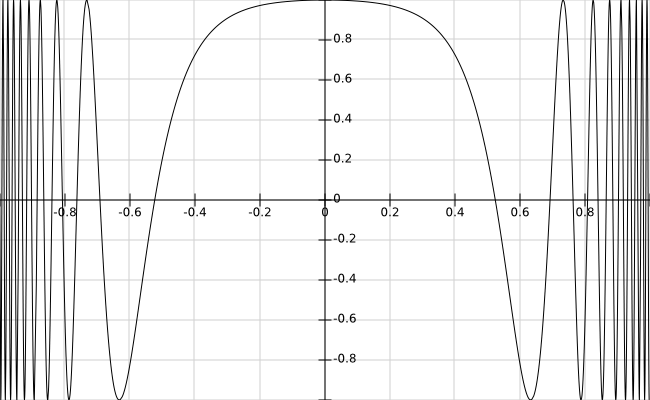
\includegraphics[width=10cm]{images/stark_oszi_funktion.png}
  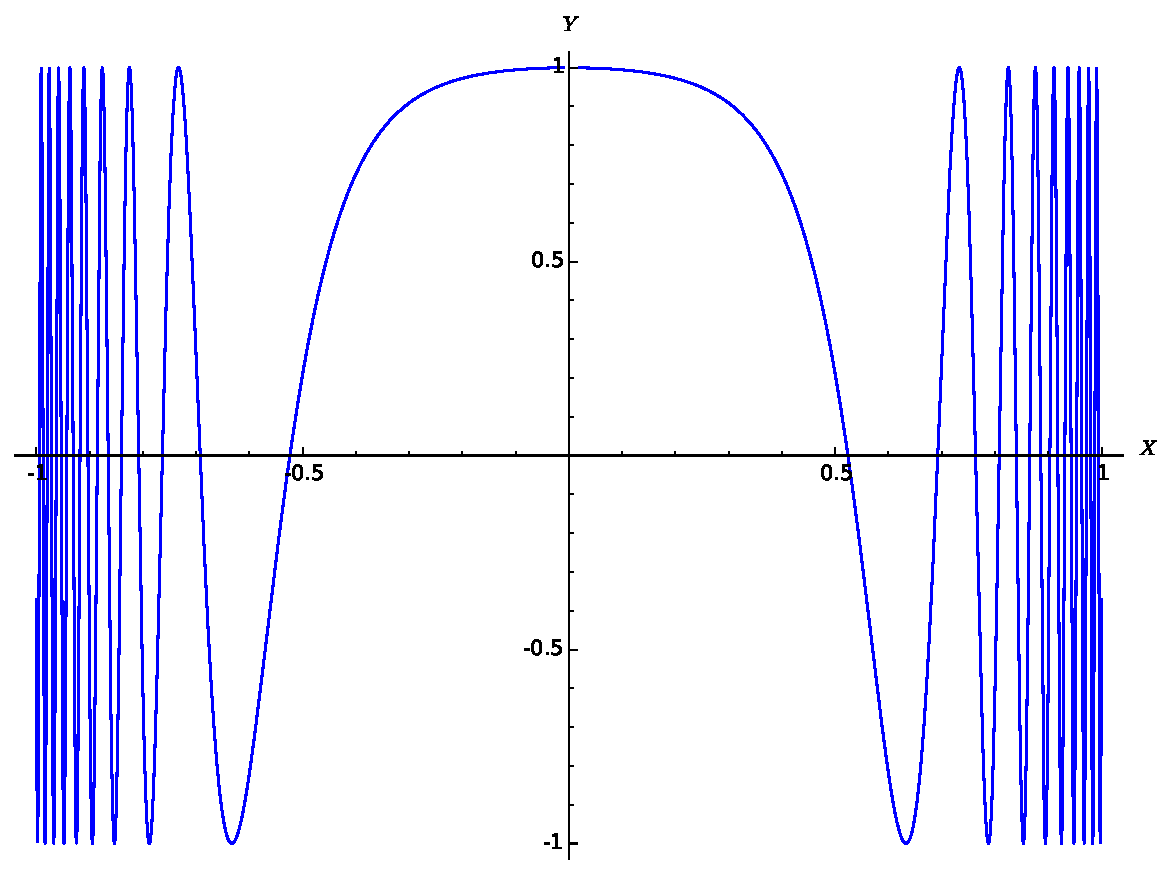
\includegraphics[width=11cm]{images/stark_oszi_funktion2.pdf}
\end{image}


%%% Local Variables:
%%% mode: latex
%%% TeX-master: "../numerik_script"
%%% End:
